\section{Investigation of weaker than expected limit for T1tttt \label{app:foundSusy}}

As shown in Fig.~\ref{fig:T1tttt_excl} the T1tttt has an observed limit $\sim 2\sigma$ weaker 
than expected. This section details studies to localise the cause of this weaker than expected
limit and to show that this is due to a fluctuation and not a systematic bias or instrumental
effect. 

As shown in Fig.~\ref{fig:T1ttttMountainRange} the bins providing 
sensitivity for T1tttt compressed and uncompressed models are $\scalht > 800$,$\geq5j$,$\eq2b$ and 
$\geq3b$. The predicted yields and observations for these as well as
adjacent \njet and \scalht bins are shown in Table~\ref{tab:yieldsExcessBins}.
The $\scalht > 800$,$\geq5j$,$\eq2b$ and $\geq3b$ bins exhibit a moderate excess. 
The adjacent bins have good data agreement with prediction implying that 
the excess is not due to a systematic bias in the prediction of these bins.

\begin{table}[h!]
  \caption{Predictions and observations for high \njet, \nb,\scalht bins}
  \label{tab:yieldsExcessBins}
  \centering
  \begin{tabular}{ lllll }
    \hline
    \hline
    \scalht & \njet & \nb & Prefit Prediction & Data\\
    \hline    
    \hline    
    $800-\infty$ & $\geq5j$ & $\geq3b$ & $0.9 \pm 0.3$  & 3 \\
    $800-\infty$ & $\geq5j$ & $2b$     & $7.2 \pm 2.2$  & 2\\
    $600-800$    & $\geq5j$ & $\geq3b$ & $1.5 \pm 0.4$  & 1 \\
    $600-800$    & $\geq5j$ & $2b$     & $10.9 \pm 2.9$ & 10 \\
    $800-\infty$ & $4j$     & $\geq3b$ & $0.1 \pm 0.0$ & 0 \\
    $800-\infty$ & $4j$     & $2b$     & $3.4 \pm 1.1$ & 2\\
    $600-800$ & $4j$     & $\geq3b$ & $0.1 \pm 0.0$ & 0 \\
    $600-800$ & $4j$     & $2b$     & $3.6 \pm 0.8$ & 7\\
    \hline
    \hline
  \end{tabular}
\end{table}

\begin{figure}[tbhp]
  \caption{Summary of predictions and data showing pre and post fit pulls for symmetric categories\label{fig:T1ttttMountainRange}} 
  \begin{center}    
    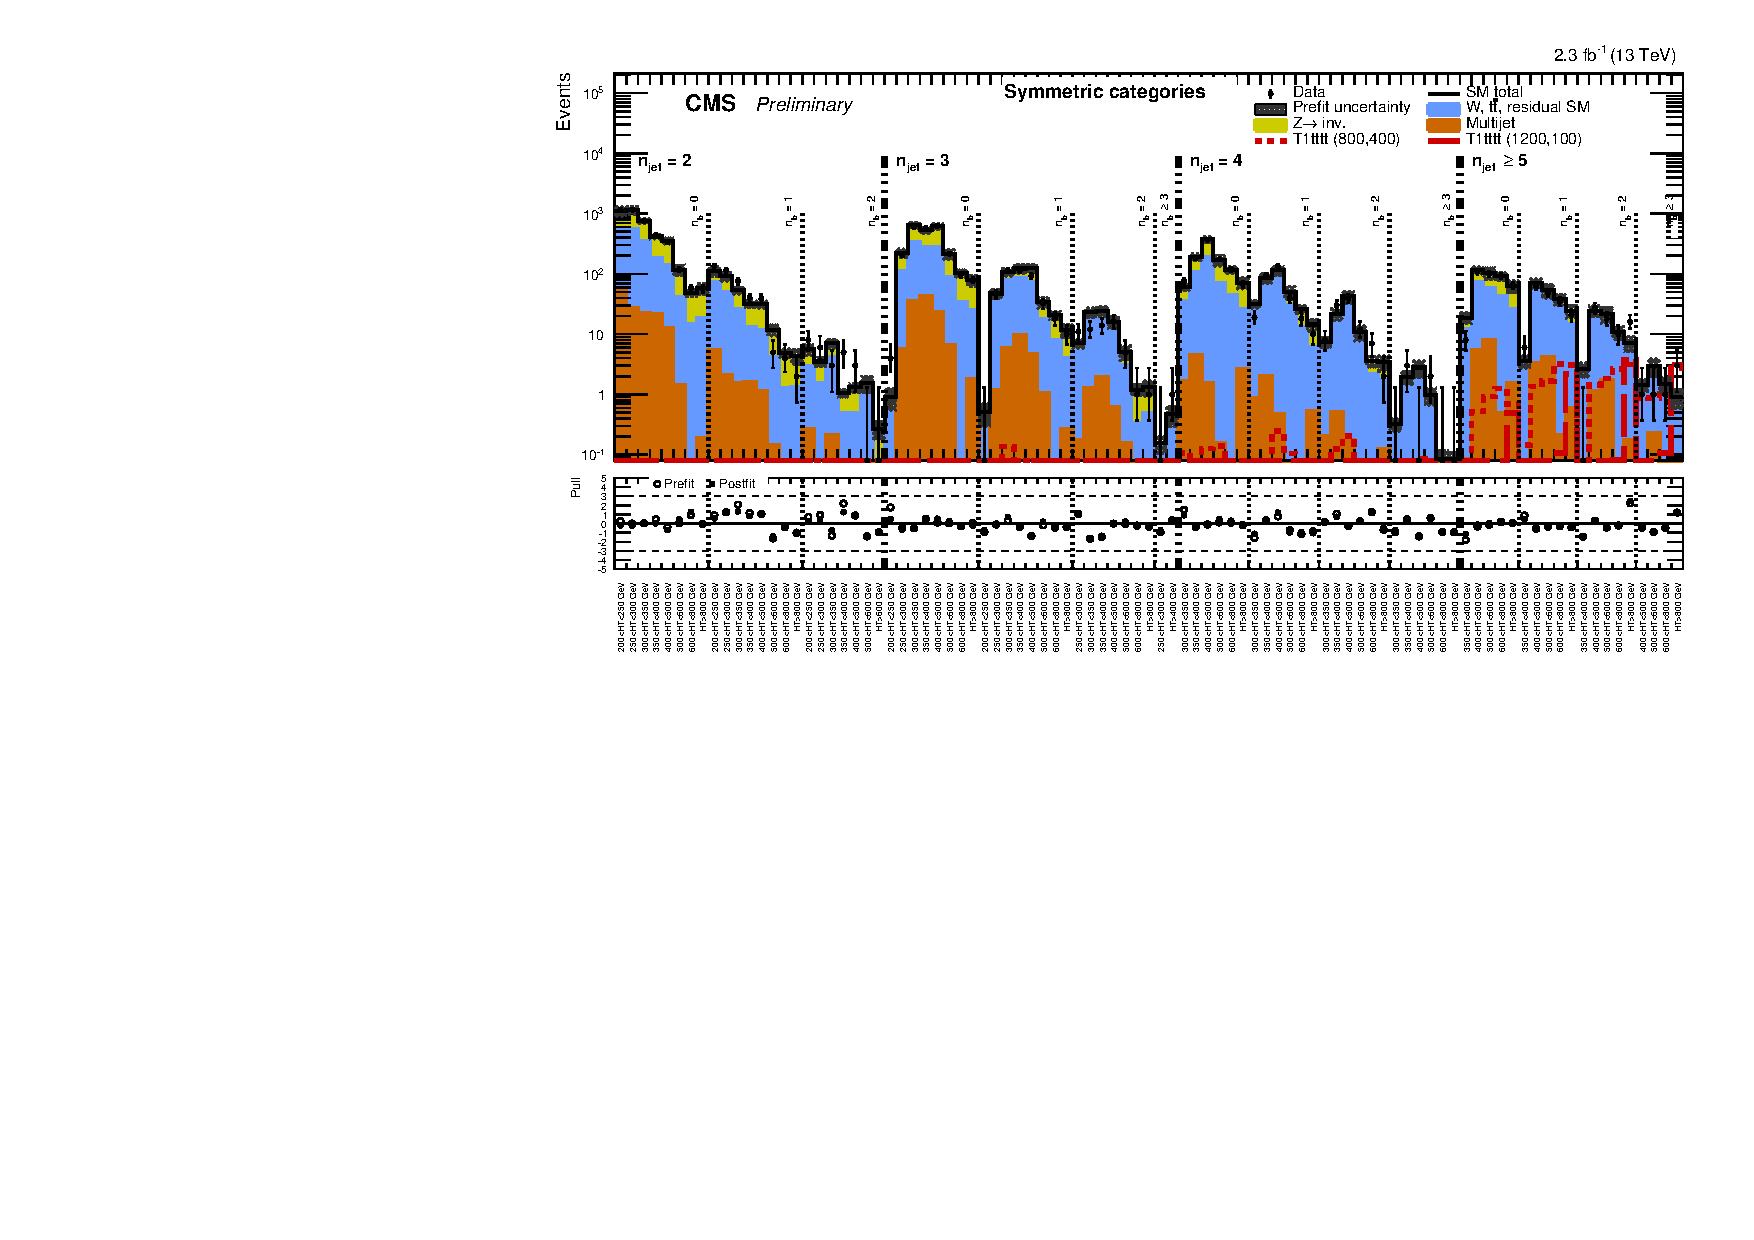
\includegraphics[width=0.8\textwidth]{figures/susyResults/summaryPlot_Symmetric_prefit_overlay_fit_b}
  \end{center}
\end{figure}

To show that the cause of the weaker than expected trend is localised to the high 
\scalht, \njet and \nb bins the excess is removed by setting the normalisation
of the \mht distribution to the observation in these bins. As shown in 
Fig.~\ref{fig:removeExcessByHand} this restores good agreement in the 
observed and expected limit, confirming these bins are resposible for the under exclusion.

\begin{figure}[tbhp]
  \caption{Limit plane for T1tttt after setting normalisation of prediction to data for bins with excess \label{fig:removeExcessByHand}} 
  \begin{center}    
    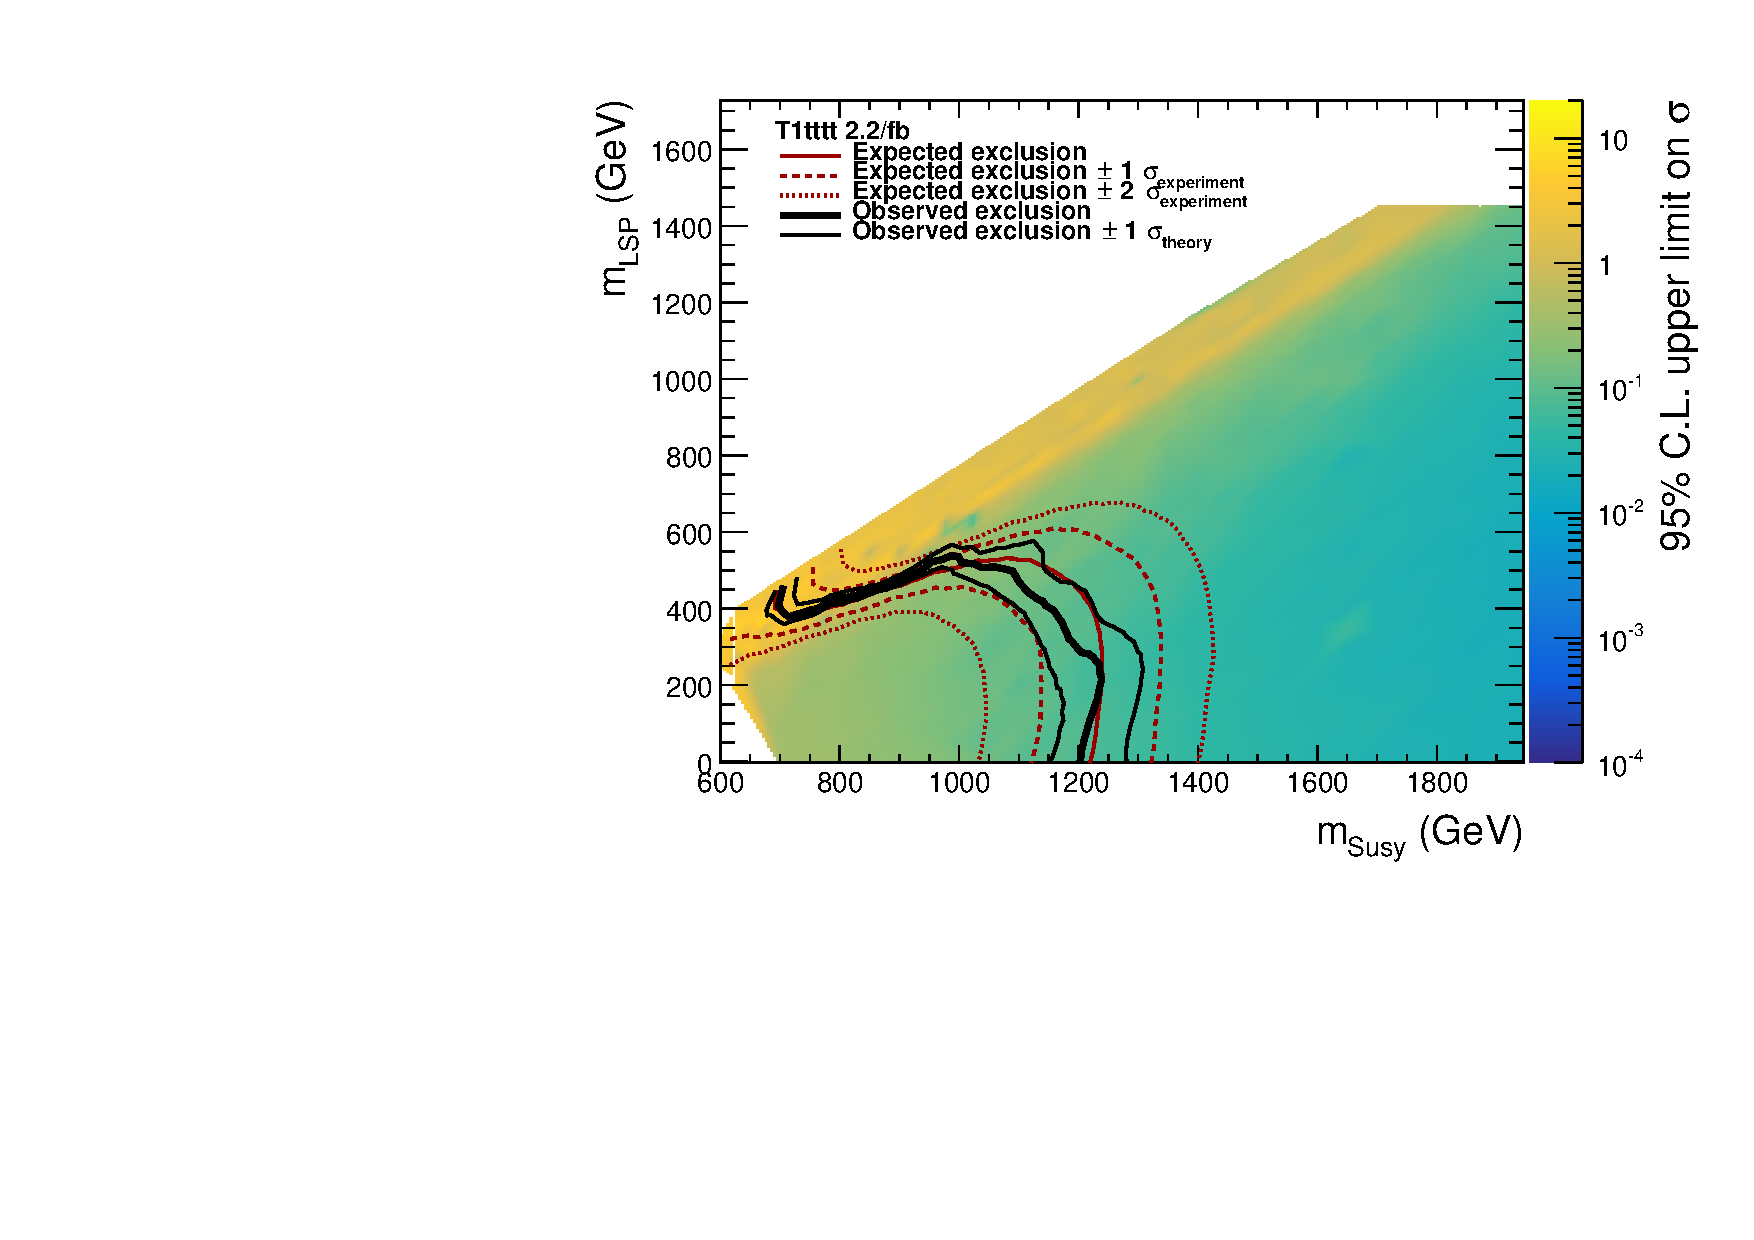
\includegraphics[width=0.8\textwidth]{figures/susyResults/finalCanvasObsLimitXs_excessRemovedByHand}
  \end{center}
\end{figure}

The \mht distribution of the data in the bins exhibiting the excess was inspected, 
as shown in Fig.~\ref{fig:mhtDistributionExcessBins} and can be seen to agree well
with prediction. Additionally, as shown in Fig.~\ref{fig:nuisPull_TemplateTtw} the template
systematic parameters are not significantly pulled for these (or any other) bins.
This provides further confirmation that the excess is due to a fluctuation in 
the Ewk background.

\begin{figure}[tbhp]
    \caption{\mht distributions for bins exhibiting excess showing good agreement between data and prediction}
      \label{fig:mhtDistributionExcessBins}}
  \begin{center}
    \subfigure[$\geq3b$]{ 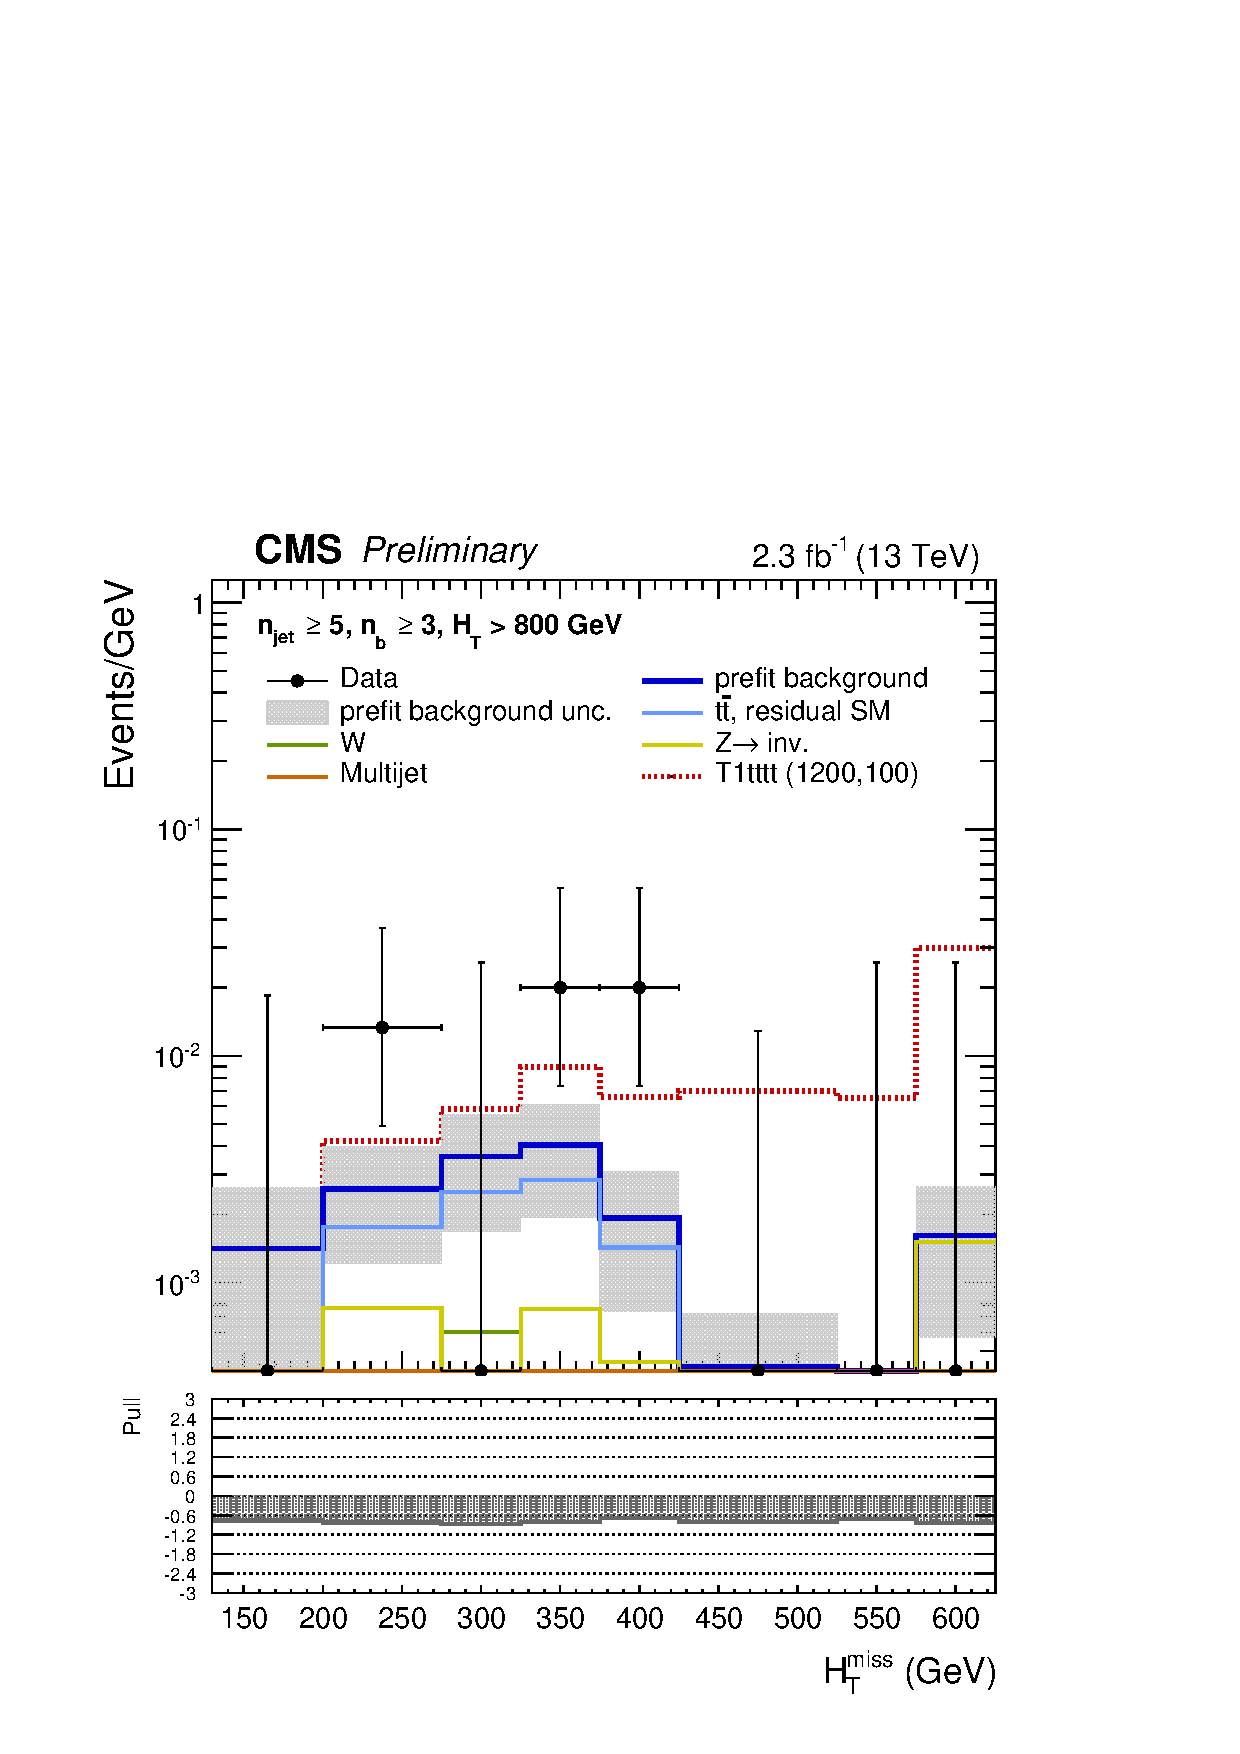
\includegraphics[width=0.45\textwidth]{figures/susyResults/postFitShape_ge3b_ge5j_800_Inf_prefit.pdf} } ~~
    \subfigure[$2b$]{ 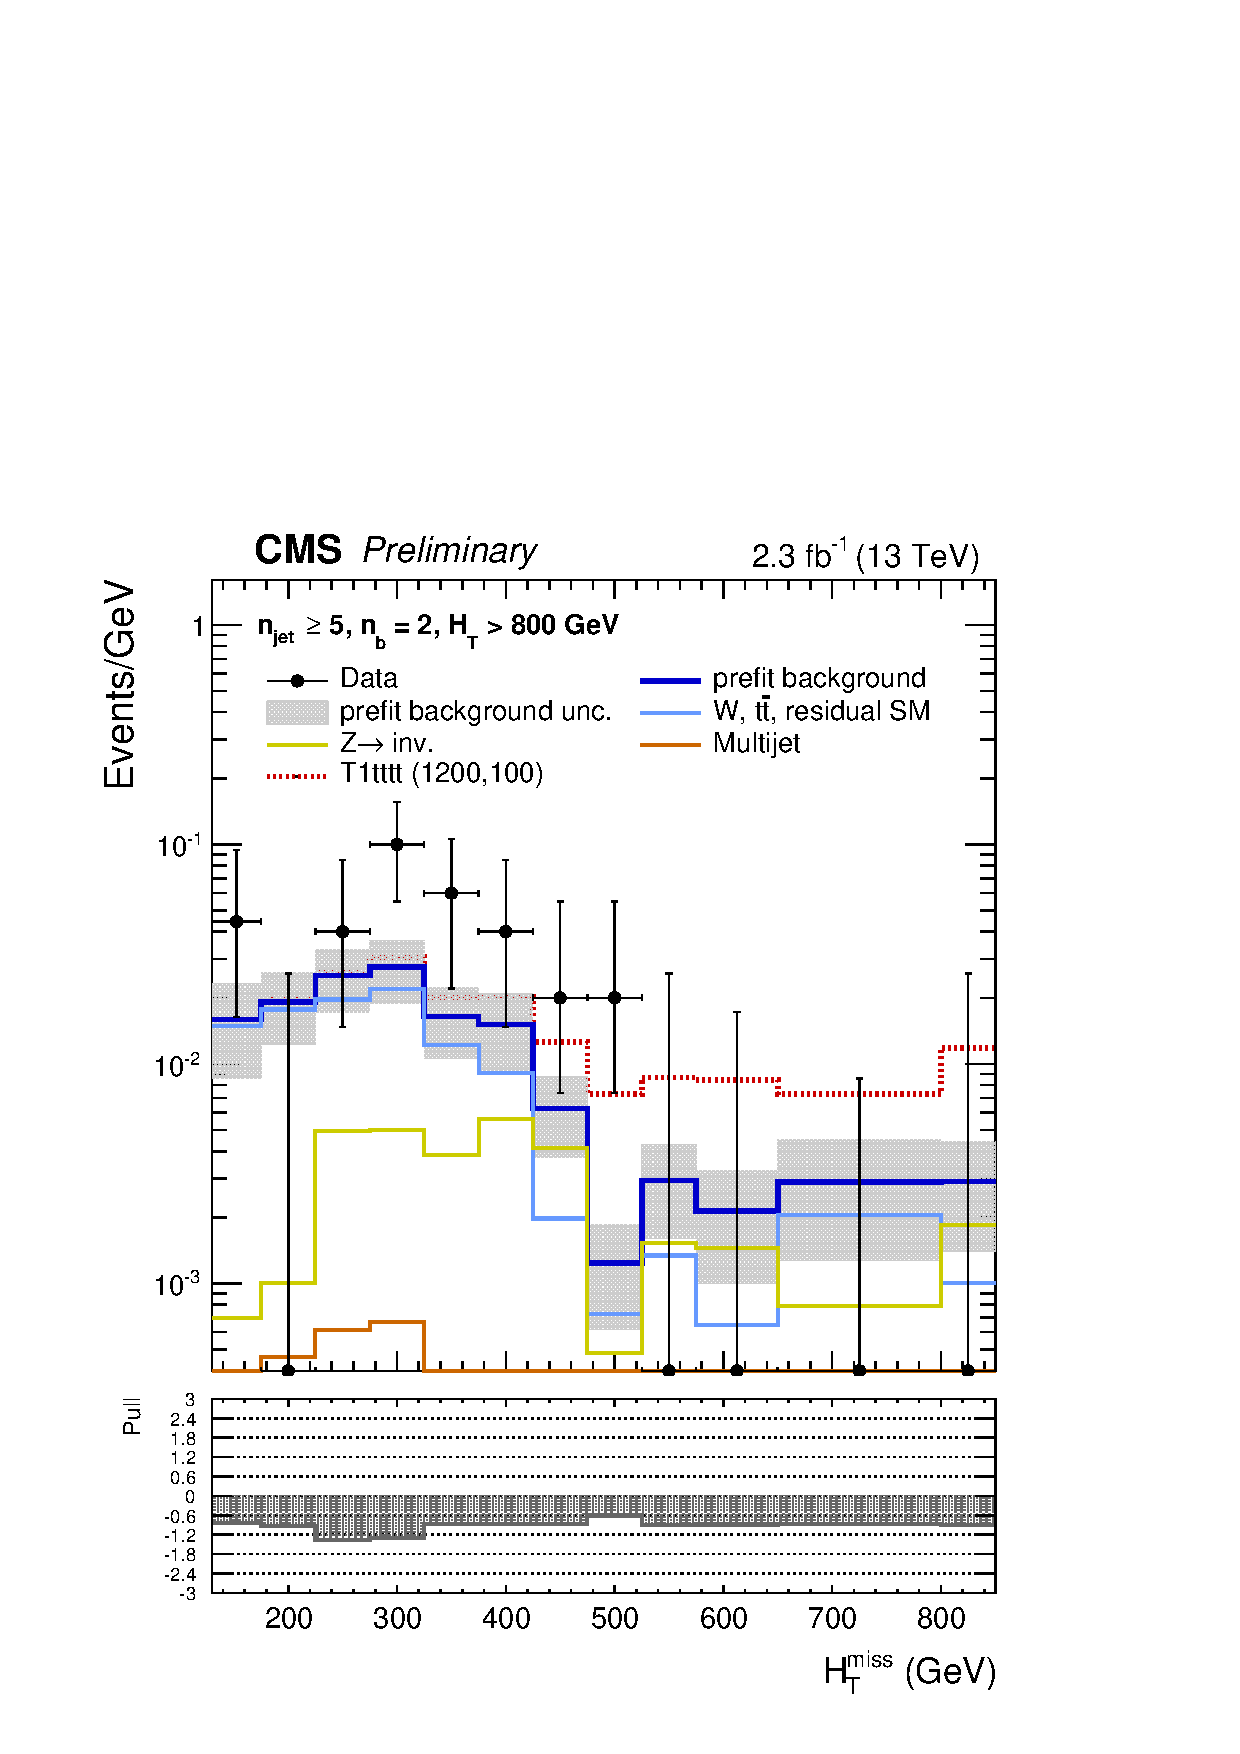
\includegraphics[width=0.45\textwidth]{figures/susyResults/postFitShape_eq2b_ge5j_800_Inf_prefit} }
  \end{center}
\end{figure}

Finally, event displays for all 19 events appearing in the $\scalht > 800$,$\geq5j$,$\ge2b$ bins
were inspected for instrumental and beam halo effects. No evidence of significant contamination
due to either of these effects were observed. In summary, no events have any sign of beam halo
around $\phi = 0,\pi$ in the muon system or calorimeters. Some events had evidence of punch 
through, however, no high \pt fake muons were created and due to the \bdphi cut the \met is
not aligned with any jet. Finally, no preferred directionality was observed in \met as shown
in Table~\ref{tab:metDirectionality}.

\begin{table}[h!]
\caption{Events in data in the bins exhibiting the excess showing no preffered directionality in \met}
\label{tab:metDirectionality}
\centering
\begin{tabular}{llllll}
PD    & run      &lumi      & event       &\met $\pt$  & \met $\phi$    \\
HTMHT & 257613   &     886  & 1374732569  &  331.808 &  174.41 \\
HTMHT & 257613   &     547  &  859340053  &  338.776 &  171.46 \\
HTMHT & 258158   &     948  & 1465719344  &  331.749 &  -86.84 \\
HTMHT & 259686   &     255  &  473615138  &  253.166 &  -23.70 \\
HTMHT & 259821   &      66  &  114171157  &  421.602 &  -87.38 \\
HTMHT & 260424   &     144  &  266740196  &  336.561 &  107.71 \\
HTMHT & 260532   &     574  &  984615795  &  256.814 &  166.67 \\
HTMHT & 260627   &     566  & 1020902998  &  192.592 &  -85.06 \\
HTMHT & 260627   &     936  & 1730280974  &  225.807 & -177.39 \\
HTMHT & 260627   &     193  &  316035428  &  220.683 &  127.35 \\
HTMHT & 258702   &     119  &  170670799  &  215.710 &  167.56 \\
HTMHT & 258177   &     658  &  966846982  &  322.483 & -155.68 \\
HTMHT & 258177   &     1151 &1639429883   & 285.055  & 94.54   \\
HTMHT & 258742   &     577  & 1038497070  &  281.241 &  -77.76 \\
JetHT & 257645   &     384  &  601397566  &  334.602 & -153.87 \\
JetHT & 258445   &       7  &    8851517  &  327.704 &    4.83 \\
JetHT & 259810   &      82  &  136409363  &  385.937 &  -52.40 \\
JetHT & 259820   &      77  &  113171056  &  104.506 &  -16.99 \\
JetHT & 260534   &     337  &  614824884  &  130.642 &  161.40
\end{tabular}
\end{table}


As an example, the event displays for a candidate punch through event is shown in 
Figures~\ref{fig:cmsShow_001}-~\ref{fig:cmsShow_003}.
For this event the hits in the muon system are located around a corner of DT and
CSC and are associated with a large energy deposit in HCAL. As can be seen
in \ref{fig:cmsShow_002}, they are also associated with an energy deposit in ECAL and tracks.
This is consistent with a punch through event.

All hits in the muon system around there are contained in the 1st
stations both in DT and CSC, as expected for a punch-through. 
If a beam-halo went through the HCAL, there should be energy deposits
aligned with the z-axis. As can be seen in Fig.~\ref{fig:cmsShow_003} the energy deposits
appear to be decently distributed and the event is not consistent with beam halo.

As the \met is not aligned with a jet it is unlikely that the punch through
significantly increased the \met in this event to bring it into selection. 
Such analysis was made of all 19 events appearing in selection for the bins
containing the excess.

In summary, no evidence for systematic bias or contamination from 
instrumental/beam halo effects was observed from the studies detailed above
and so the excess is concluded to be due to a statistical fluctuation 
in two bins at high \njet, \nb and \scalht. 

\begin{figure}[tbhp]
  \caption{Event display for run 259810, lumi 82, event 136409363 (summary view)}
  \label{fig:cmsShow_001}
  \begin{center}    
    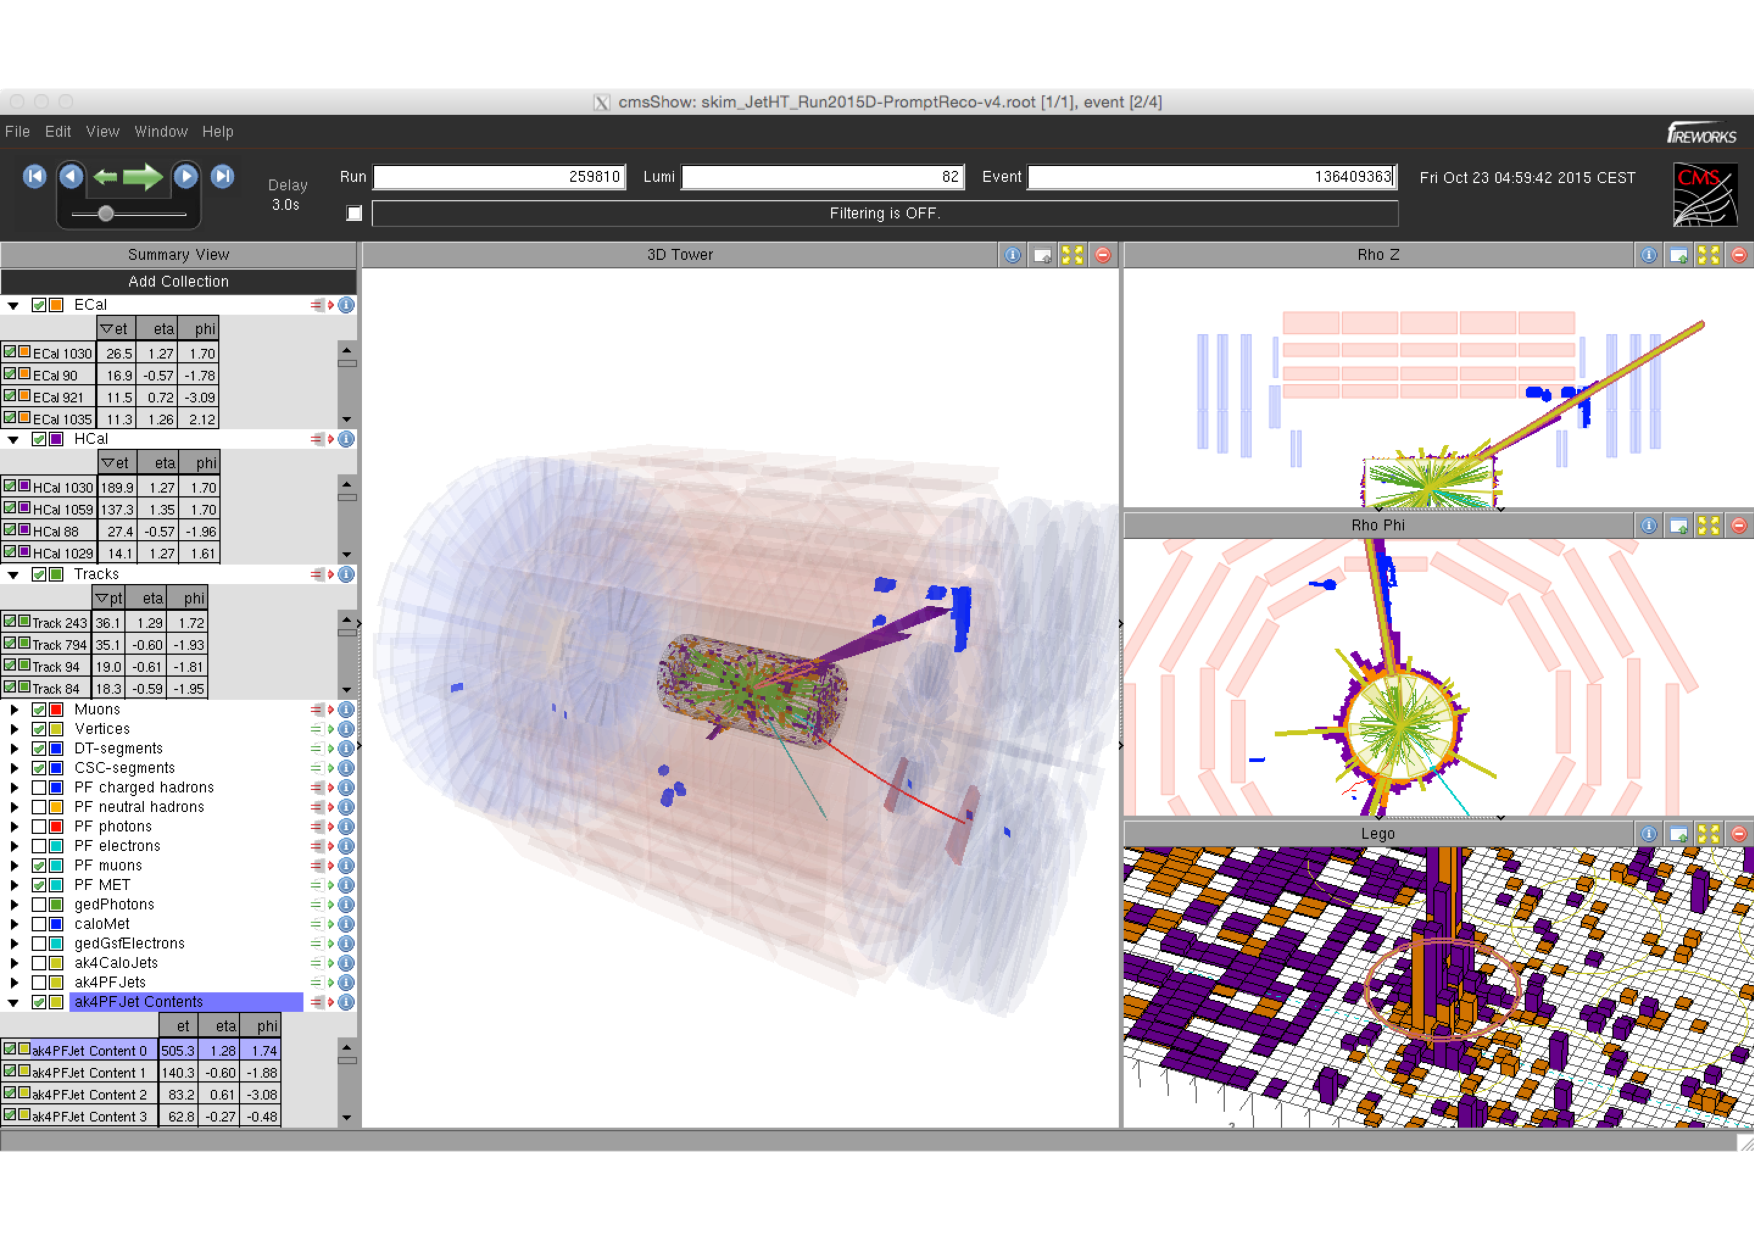
\includegraphics[width=0.8\textwidth]{figures/susyResults/cmsShow_001}
  \end{center}
\end{figure}
\begin{figure}[tbhp]
  \caption{Event display for run 259810, lumi 82, event 136409363 (3D tower view)}
  \label{fig:cmsShow_002}
  \begin{center}    
    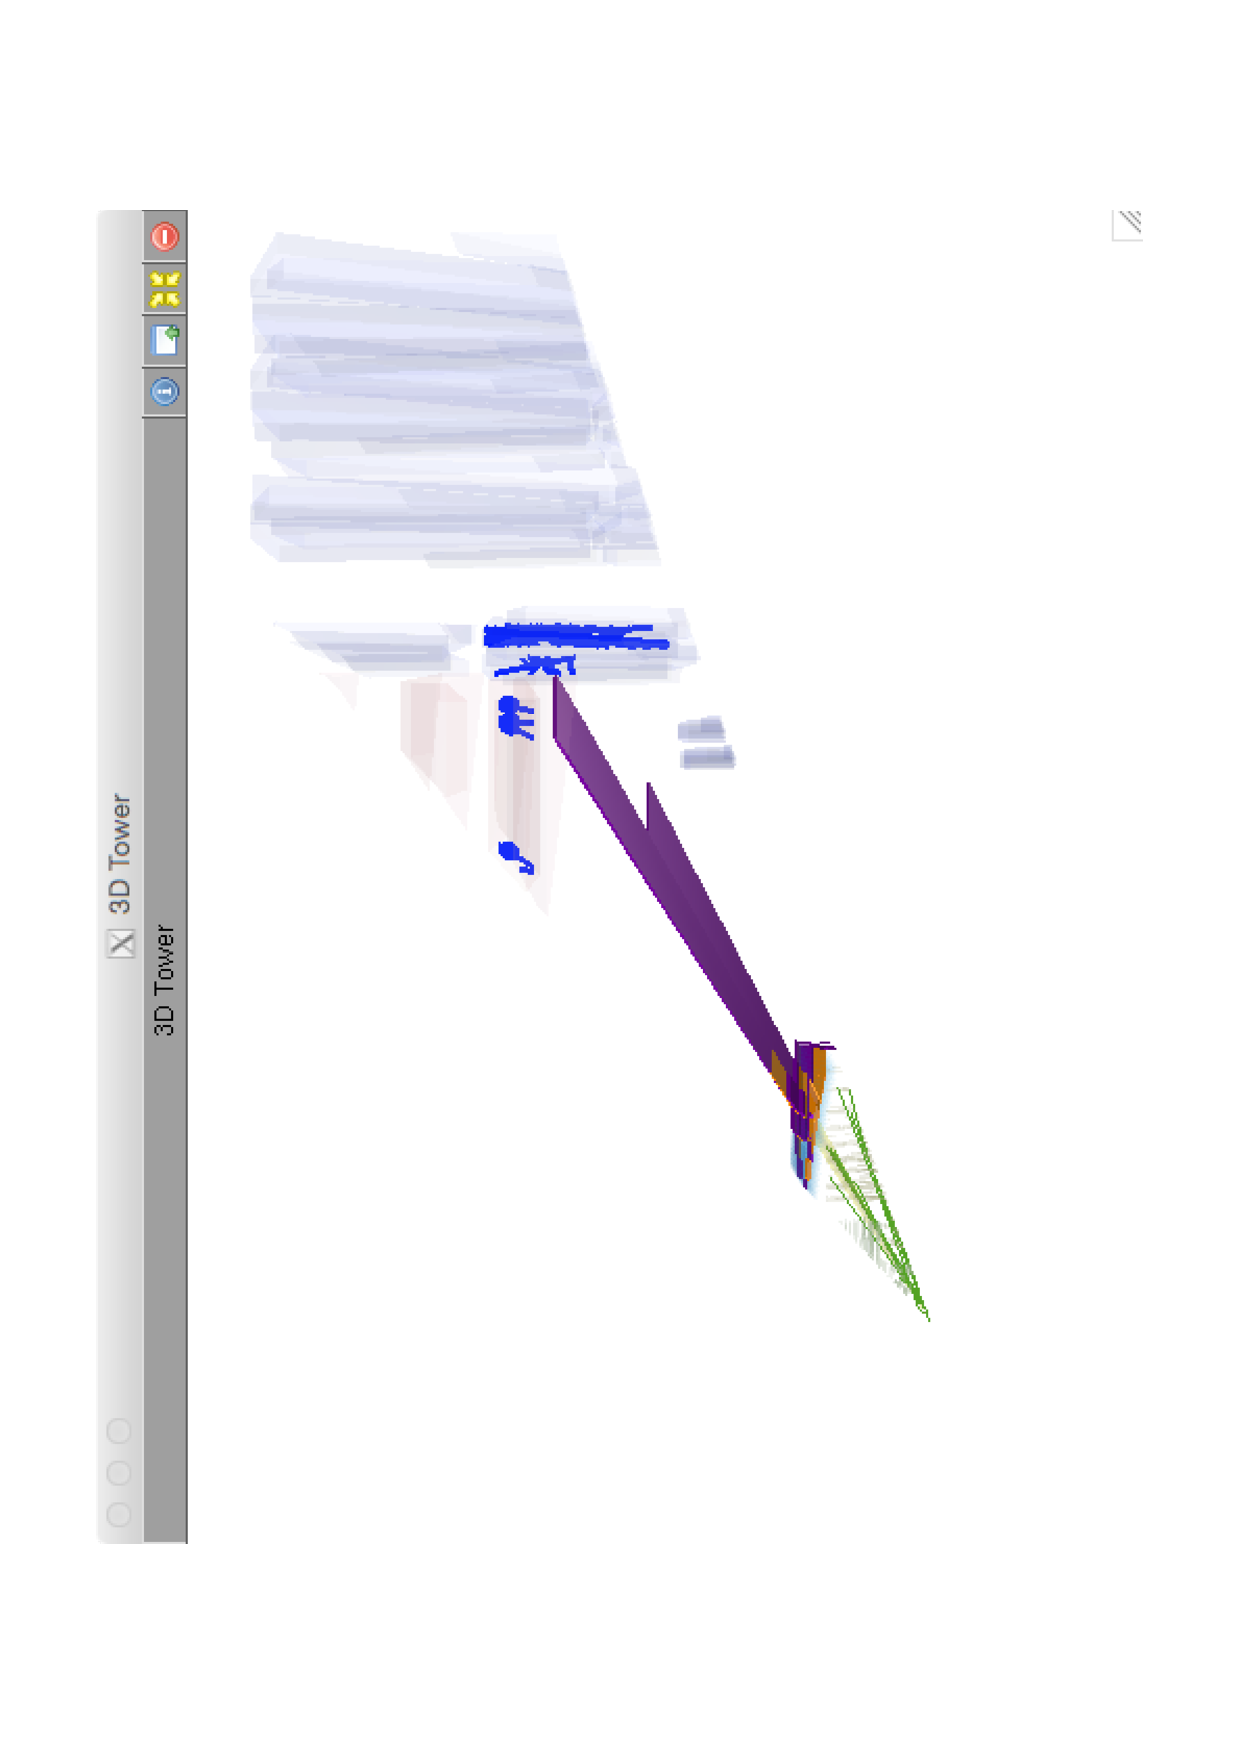
\includegraphics[width=0.8\textwidth]{figures/susyResults/cmsShow_002}
  \end{center}
\end{figure}
\begin{figure}[tbhp]
  \caption{Event display for run 259810, lumi 82, event 136409363 (HCAL detail view)}
  \label{fig:cmsShow_003}
  \begin{center}    
    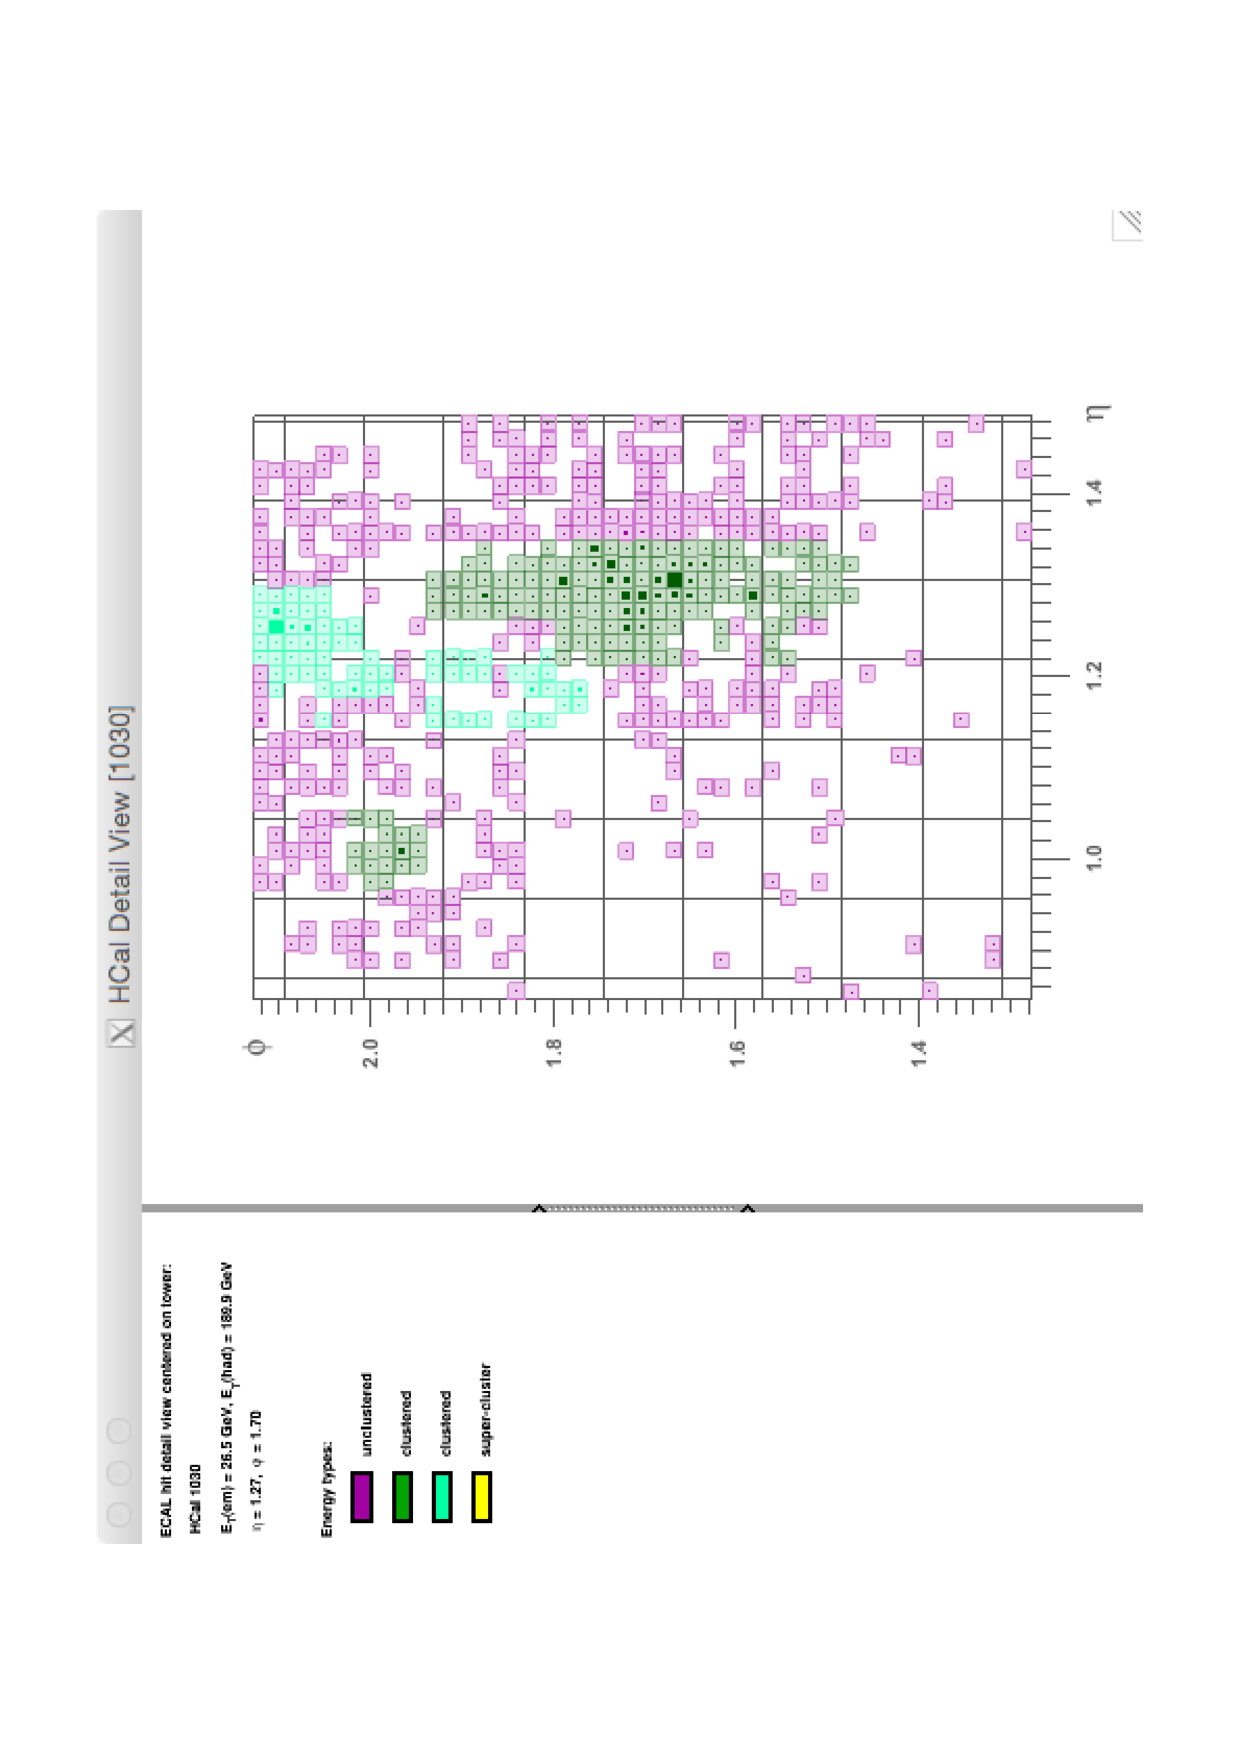
\includegraphics[width=0.8\textwidth]{figures/susyResults/cmsShow_003}
  \end{center}
\end{figure}
